\documentclass[11pt, oneside]{article}   	% use "amsart" instead of "article" for AMSLaTeX format
\usepackage{geometry}                		% See geometry.pdf to learn the layout options. There are lots.
\usepackage{graphicx}
\usepackage{amsmath}				% Use for matrices

\geometry{letterpaper}                   		% ... or a4paper or a5paper or ... 

%\geometry{landscape}                		% Activate for rotated page geometry
%\usepackage[parfill]{parskip}    		% Activate to begin paragraphs with an empty line rather than an indent
\usepackage{graphicx}				% Use pdf, png, jpg, or eps§ with pdflatex; use eps in DVI mode
								% TeX will automatically convert eps --> pdf in pdflatex		
\usepackage{amssymb}

%SetFonts

%SetFonts


\title{Homework 1 \\
	\large EECE 5550}
\author{Andrew Tu}
\date{\today}							% Activate to display a given date or no date

\begin{document}
\maketitle
\newpage
%\section{}
%\subsection{}

\section{2}

\subsection{Visual of Workspace}
\begin{figure}[h]
   \centering
   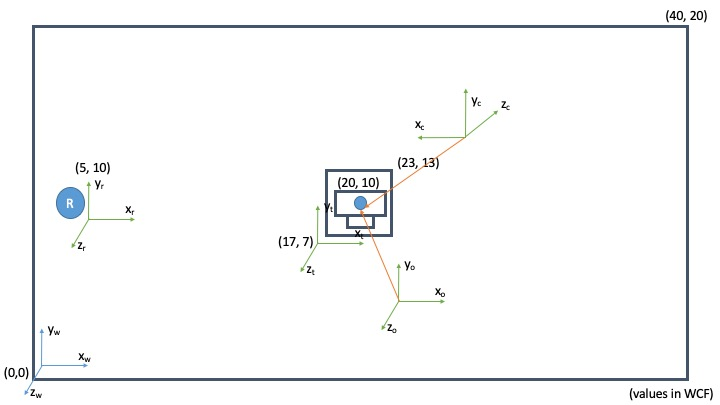
\includegraphics[width=.75\textwidth]{../layout/top_down.jpg} % requires the graphicx package
   \caption{Top Down Image of Room.}
   \label{fig:top_down}
\end{figure}

\begin{figure}[h]
   \centering
   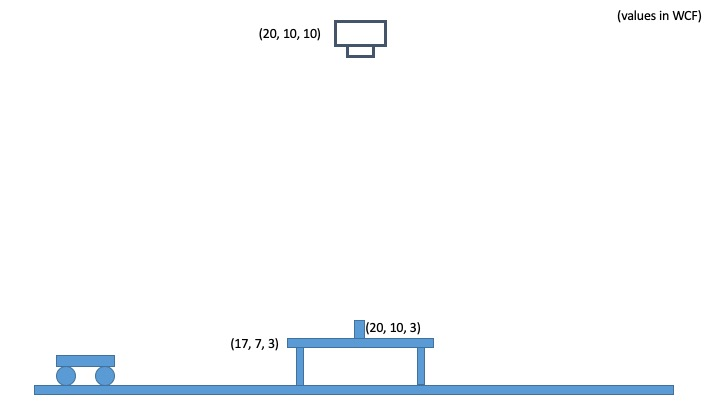
\includegraphics[width=.75\textwidth]{../layout/side.jpg} % requires the graphicx package
   \caption{Side Image of Room.}
   \label{fig:side}
\end{figure}


\subsection{Assign Coordinate Frames}
See fig. \ref{fig:top_down}.
Assign the world, robot, camera, table, and object coordinate frames.
\begin{itemize}
  \item world: origin at top left
  \item robot: origin at $(5, 10, 0)_{world}$
  \item camera: origin at $(20, 10, 10)_{world}$
  \item table: origin at $(23, 7, 3)_{world}$
  \item object: origin at $(20, 10, 3)_{world}$
\end{itemize}

\subsection{Express Homogeneous Transforms}
$$ T_s^d = 
\begin{bmatrix} 
r_{11} & r_{21} & r_{31} & dx \\
r_{12} & r_{22} & r_{32} & dy \\
r_{13} & r_{23} & r_{33} & dz \\
0 & 0 & 0 & 1 \\
\end{bmatrix}
$$
\subsubsection{Robot coordinate frame with respect to the world coordinate frame}
$$ T_r^w = 
\begin{bmatrix} 
1 & 0 & 0 & 5 \\
0 & 1 & 0 & 10 \\
0 & 0 & 1 & 0 \\
0 & 0 & 0 & 1 \\
\end{bmatrix}
$$
\subsubsection{Table coordinate frame with respect to the world coordinate frame}
$$ T_t^w =
\begin{bmatrix} 
1 & 0 & 0 & 17 \\
0 & 1 & 0 & 7 \\
0 & 0 & 1 & 3 \\
0 & 0 & 0 & 1 \\
\end{bmatrix}
$$
\subsubsection{Camera coordinate frame with respect to the table coordinate frame}
$$
T_c^t =
\begin{bmatrix} 
-1 & 0 & 0 & 3 \\
0 & 1 & 0 & 3 \\
0 & 0 & -1 & 7 \\
0 & 0 & 0 & 1 \\
\end{bmatrix}
$$
\subsubsection{Object coordinate frame with respect to the table coordinate frame}
$$ T_o^t =
\begin{bmatrix} 
1 & 0 & 0 & 3 \\
0 & 1 & 0 & 3 \\
0 & 0 & 1 & 0 \\
0 & 0 & 0 & 1 \\
\end{bmatrix}
$$
\subsubsection{Object coordinate frame with respect to robot coordinate frame}
$$ T_o^r = 
\begin{bmatrix} 
1 & 0 & 0 & 15 \\
0 & 1 & 0 & 0 \\
0 & 0 & 1 & 3 \\
0 & 0 & 0 & 1 \\
\end{bmatrix}
$$

\subsection{General Equation from Object in Robot Coordinate to rest of coordinate frames}
$$
p_o^r = 
\begin{bmatrix}
15\\
0\\
3\\
1
\end{bmatrix}
$$

$$
P_o^f =  \underset{4\times4}{T_w^f} * \underset{4\times4}{T_r^w} * \underset{4\times1}{p_o^r}
$$

\subsection{Experimentation}
\begin{figure}[h]
   \centering
   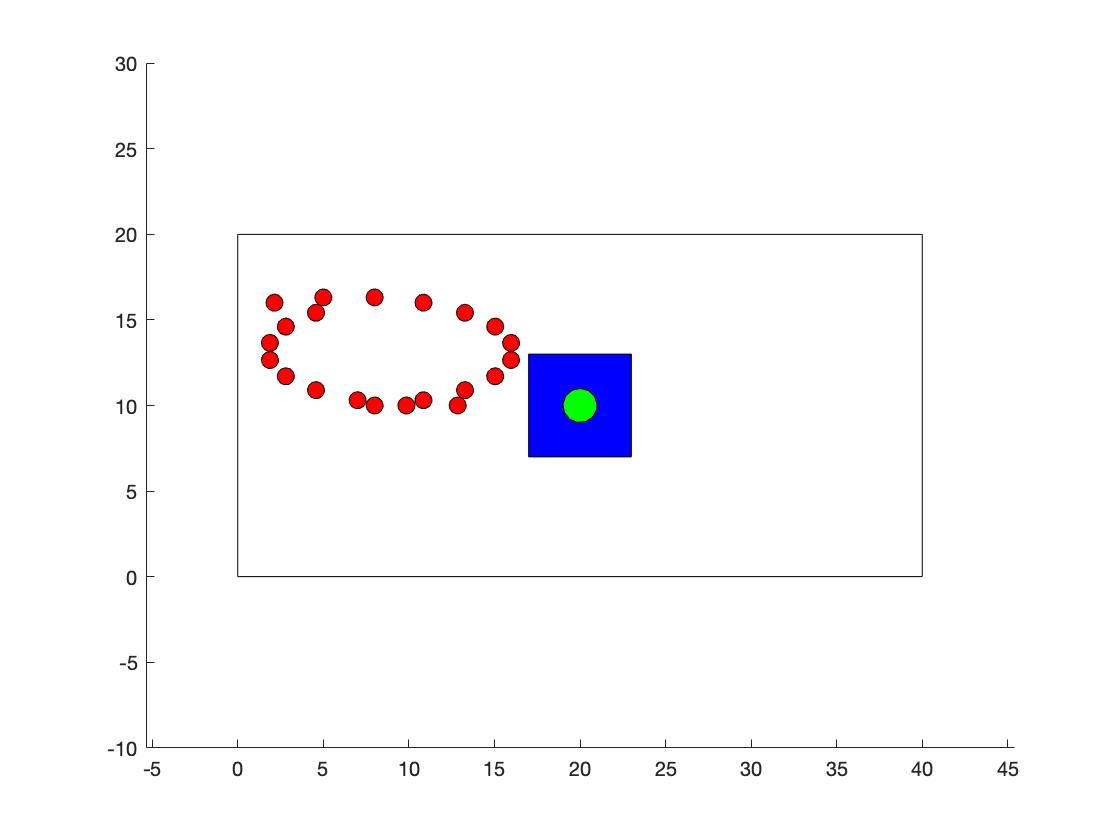
\includegraphics[width=.5\textwidth]{../experiments.jpg} % requires the graphicx package
   \caption{Experiments with Transition Matrix}
   \label{fig:exp}
\end{figure}



\end{document}  